\begin{pastexam}[label={px:gk3-102-ds-01}]{高考三級資訊處理 102 年 第一題}
（申論；22 分）

將整數資料 80, 40, 19, 120, 94, 110, 115, 90, 88, 92, 98 依序存入一棵空的二元搜尋樹
（binary search tree）。
\begin{enumerate}[leftmargin=2.6em, labelsep=0.4em]
\item[㈠] 請畫出完成資料輸入的二元搜尋樹。（6 分）
\item[㈡] 從㈠產生的二元搜尋樹中刪除（delete）資料 94，請畫出完成刪除動作後的二元搜尋樹。
（給出一個正確樹即可）（6 分）
\item[㈢] 請寫出自二元搜尋樹找到最大值資料所在節點（node）的演算法。（10 分）
\end{enumerate}
\end{pastexam}

\begin{pastsoln}
\textbf{㈠} 插入的規則（資結書第~9.2~節）：從根開始，比目前節點小往左、大往右，走到空的位置
就放下。 逐筆插入：
\begin{center}
\small
\begin{tabular}{cl}
\toprule
插入 & 走過的路徑與位置 \\
\midrule
80 & 樹是空的，當根 \\
40 & $40 < 80$，80 的左子 \\
19 & $19 < 80$、$19 < 40$，40 的左子 \\
120 & $120 > 80$，80 的右子 \\
94 & $94 > 80$、$94 < 120$，120 的左子 \\
110 & $110 > 80$、$< 120$、$> 94$，94 的右子 \\
115 & $115 > 80$、$< 120$、$> 94$、$> 110$，110 的右子 \\
90 & $90 > 80$、$< 120$、$< 94$，94 的左子 \\
88 & $88 > 80$、$< 120$、$< 94$、$< 90$，90 的左子 \\
92 & $92 > 80$、$< 120$、$< 94$、$> 90$，90 的右子 \\
98 & $98 > 80$、$< 120$、$> 94$、$< 110$，110 的左子 \\
\bottomrule
\end{tabular}
\end{center}
完成後的樹：
\begin{center}
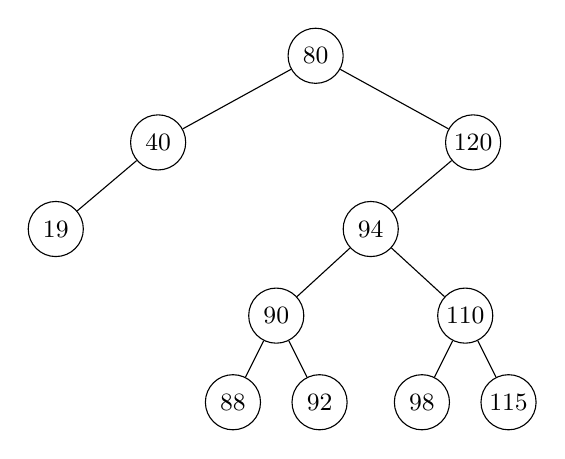
\begin{tikzpicture}[n/.style={circle,draw,inner sep=0pt,minimum size=7mm,font=\small},
  level distance=11mm, level 1/.style={sibling distance=40mm}, level 2/.style={sibling distance=26mm},
  level 3/.style={sibling distance=24mm}, level 4/.style={sibling distance=11mm}]
\node[n] {80}
  child {node[n] {40} child {node[n] {19}} child[missing]}
  child {node[n] {120}
    child {node[n] {94}
      child {node[n] {90} child {node[n] {88}} child {node[n] {92}}}
      child {node[n] {110} child {node[n] {98}} child {node[n] {115}}}}
    child[missing]};
\end{tikzpicture}
\end{center}
中序走訪是 19, 40, 80, 88, 90, 92, 94, 98, 110, 115, 120，由小到大，可以拿來檢查樹畫得對不對。

\textbf{㈡} 94 有兩個子節點，不能直接拿掉。 做法（資結書虛擬碼~9.7）：用它的中序後繼，也就是右子樹
裡最小的數，來頂替。 94 的右子樹根是 110，一路往左走到 98，98 沒有左子，所以後繼是 98。
98 是葉節點，把它從原位置拿掉，再把 94 那個節點的值改成 98：
\begin{center}
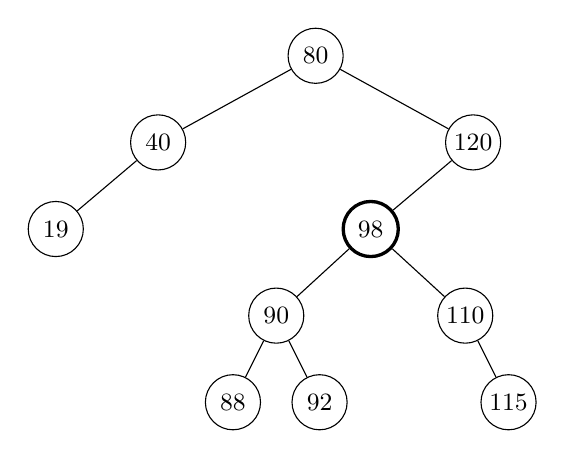
\begin{tikzpicture}[n/.style={circle,draw,inner sep=0pt,minimum size=7mm,font=\small},
  level distance=11mm, level 1/.style={sibling distance=40mm}, level 2/.style={sibling distance=26mm},
  level 3/.style={sibling distance=24mm}, level 4/.style={sibling distance=11mm}]
\node[n] {80}
  child {node[n] {40} child {node[n] {19}} child[missing]}
  child {node[n] {120}
    child {node[n,very thick] {98}
      child {node[n] {90} child {node[n] {88}} child {node[n] {92}}}
      child {node[n] {110} child[missing] child {node[n] {115}}}}
    child[missing]};
\end{tikzpicture}
\end{center}
題目說給一個正確的樹即可。 改用中序前驅（左子樹最大的 92）頂替也對，那時 92 換到 94 的位置，
90 只剩左子 88，110 底下仍是 98 和 115。 兩種結果的中序走訪都是原來的序列去掉 94。

\textbf{㈢} 二元搜尋樹裡，任何節點右子樹的值都比它大，所以只要還有右子，最大值就在右邊。 從根開始
一直往右子走，走到沒有右子的節點，那個節點就是最大值（資結書虛擬碼~9.3）。
\begin{pseudo}{找最大值所在的節點}
\Function{Tree-Maximum}{$x$} \Comment{$x$ 指向樹根}
    \If{$x = \NIL$}
        \State \Return \NIL \Comment{空樹沒有最大值}
    \EndIf
    \While{$x.\mathit{right} \ne \NIL$}
        \State $x \gets x.\mathit{right}$
    \EndWhile
    \State \Return $x$
\EndFunction
\end{pseudo}
正確性：設迴圈停在節點 $x$。 從根到 $x$ 每一步都往右走，所以路上每個節點和它左子樹的值都比
$x$ 小；$x$ 沒有右子，它左子樹的值也比 $x$ 小。 樹裡每個節點不是在這條路上，就是在路上某個
節點（含 $x$）的左子樹裡，所以 $x$ 最大。 時間是 $O(h)$，$h$ 是樹高：平衡時 $O(\log n)$，
退化成一條鏈時 $O(n)$。 以㈠的樹為例，路徑是 $80 \to 120$，120 沒有右子，最大值是 120。
\end{pastsoln}
